\documentclass[a4paper,notitlepage,parskip=half,plainheadsepline]{scrartcl}

\usepackage{silence}
\WarningsOff[everypage]% Suppress warnings related to package everypage
\usepackage{snapshot} 
\usepackage{scrlayer-scrpage} 
\usepackage{iftex}
\usepackage[ngerman]{babel}
\usepackage{graphicx}
\usepackage{float}
\usepackage[T1]{fontenc}
\usepackage[utf8]{inputenc}
\usepackage{pifont}
\usepackage{amsmath}
\usepackage[german]{varioref}
\usepackage[text={6.8in,9.6in},top=0.8in,centering]{geometry}
\usepackage{datetime2}
\usepackage{array,multirow,tabularx}
\usepackage{listingsutf8}
\usepackage[table,svgnames,dvipsnames]{xcolor}
\usepackage[most,breakable,skins,listingsutf8]{tcolorbox}
%\tcbuselibrary{listingsutf8}
\usepackage[color=blue!90,scale=0.8,placement=bottom,vshift=1.2cm]{background}
\usepackage{array}

%%%%%%%%%%%%%%%%%%%%%%%%%%%%%%%%%%%%%%%%%%          Aufgabe oder Loesung 
\newif\ifloesung
%\loesungtrue
\loesungfalse
%%%%%%%%%%%%%%%%%%%%%%%%%%%%%%%%%%%%%%%%%%%%%%%%%%%%%%%%%%%%%%%%%%%%%%%%%


%\backgroundsetup{contents={Version vom \today}}
\backgroundsetup{contents={Version vom \today}}
%\pagestyle{empty}

\pagestyle{scrheadings}
\clearpairofpagestyles
\ihead{Fachinformatiker Anwendungsentwickler~/~Informatik--Studenten}
\chead{}
\ohead{C--Programmierung}
\ifoot{Frank Zimmermann}
\cfoot{SVLFG}
\ofoot{}
\ofoot{\pagemark}

\graphicspath{{./jpg/}}
\DeclareGraphicsExtensions{.jpg,.eps,.png}
%\usepackage{courier}

\newcommand{\mingw}{\textsl{MinGW}}
\newcommand{\bash}{\emph{bash}}
\newcommand{\msys}{\textsl{MSYS}}
\newcommand{\gcc}{\emph{gcc}}
\newcommand{\git}{\emph{Git}}
\newcommand{\listingsfont}{\ttfamily}

\RedeclareSectionCommand[
  beforeskip=-1\baselineskip,
  afterskip=.5\baselineskip]{section}
\RedeclareSectionCommand[
  beforeskip=-.75\baselineskip,
  afterskip=.5\baselineskip]{subsection}
\RedeclareSectionCommand[
  beforeskip=-.5\baselineskip,
  afterskip=.25\baselineskip]{subsubsection}
\RedeclareSectionCommand[
  beforeskip=.5\baselineskip,
  afterskip=-1em]{paragraph}
\RedeclareSectionCommand[
  beforeskip=-.5\baselineskip,
  afterskip=-1em]{subparagraph}

% Wenn pdflatex benutzt wird sollen die 
% installierten! frutiger-Fonts verwendet werden
% Ansonsten die TeX-eigenen cmbright
\ifPDFTeX %
\usepackage[scaled=0.90]{frutiger}
\renewcommand\familydefault{\sfdefault}
%\DeclareFixedFont\ott{T1}{phv}{mc}{n}{10pt
\else
\usepackage{cmbright}
\fi

\newfont{\lf}{svlfg scaled 2000}%
\newcolumntype{P}[1]{>{\centering\arraybackslash}p{#1}}

\ifloesung
\newtcbinputlisting[auto counter,list inside=lol,list type={lstlisting}]{\mylisting}[3][]{%
  toptitle=2mm,
  bottomtitle=2mm,listing only,
  colback=lightgray,
  %colback=yellow!10,
  listing file={#3},
  listing options={language=c,
  aboveskip=5pt,
  belowskip=5pt,
  columns=flexible,
  keywordstyle=\color{blue},
  basicstyle=\footnotesize\listingsfont},
  colback=white,
  %colframe=gray!75!black,
  colframe=yellow!50!black,
  listing only,
  fonttitle=\bfseries,
  breakable,
  %title={Soubor \thetcbcounter: #2},
  title=Musterlösung für \texttt{#3},
  #1
}
\fi



\begin{document}
\tcbset{enhanced,colback=green!5!white, boxrule=0.5pt, colframe=green!35!black,fonttitle=\bfseries\Large}
        % \begin{tcolorbox}[drop lifted shadow]
        % This is a tcolorbox.
        % \end{tcolorbox}\par\bigskip
        \begin{tcolorbox}[toptitle=3mm,bottomtitle=3mm,title=\centering{{\lf J}\hfil Ausbildung Fachinformatiker Anwendungsentwicklung\hfil {\lf J}},
          drop lifted shadow=gray]
        \centering{\vspace{0.5cm}\LARGE Programmierübung %
        \ifloesung (mit Musterlösung)\fi}\\[0.3cm]
        \centering{C--Programmierung}\\\vspace{0.5cm}
        \end{tcolorbox}

\section{Aufgabe}
Es ist ein Programm (\texttt{myfilter.c}) zu schreiben, das den Namen einer beliebigen Text--Datei/Pfad

\begin{enumerate}
\item als Parameter einliest,
\item diese Datei öffnet,
\item deren Inhalt einliest,
\item bestimmte Operationen ausführt und
\item das Ergebnis in die Standard--Ausgabe schreibt.
\end{enumerate}

Der Datei/Pfadname kann entweder ohne Parameterkennzeichnung übergeben werden oder mit einer Parameterkennzeichnung (\texttt{myfilter -i <inputfile>} oder \texttt{myfilter <inputfile>}). Weitere optionale Parameter müssen von dem Programm eingelesen werden können. Die Parameter bestehen jeweils aus einem Buchstaben und sind durch ein vorangestelltes \texttt{-} gekennzeichnet. Diese Parameter bestimmen, welche von den u.g. Operationen ausgeführt werden sollen. Werden keine optionalen Parameter eingegeben, so soll eine \texttt{usage()}--Meldung ausgegeben werden (\texttt{./myfilter [-c|-w|-l] [-i] inputfile}). Folgende Operationen sollen durch das Programm durchgeführt werden können:

\begin{center}
\begin{tabular}{|P{5cm}|P{6cm}|P{4cm}|}\hline
Parameter  & Operation & Ausgabe\\\hline
kein & mache garnichts & \texttt{usage()} ausgeben\\
-c   & Zähle alle Zeichen& {\texttt Zeichen=nnnn}\\
-w   & Zähle alle Wörter& {\texttt Wörter=nnnn}\\
-l   & Zähle alle Zeilen & {\texttt Zeilen=nnnn} \\\hline
\end{tabular}
\end{center}

Das Programm soll so konzipiert werden, dass später gegebenenfalls weitere optionale Parameter leicht hinzuzufügen sind.
Außerdem soll das Programm als \emph{Filter} arbeiten können, d.h. falls kein Datei oder Pfadname als Parameter angegeben wurde, soll das Programm seine Eingabe aus dem Kanal Standard--Eingabe beziehen. Das Programm soll seine Ausgabe immer in die Standard--Ausgabe schreiben.
Einige mögliche Aufrufe könnten z.B. folgendermaßen aussehen:
% Das Programm soll in reinem (Standard--) C geschrieben werden und sowohl auf der NT4 (Visual C++ oder eigener vorhandener Schul-Compiler) als auch auf der Linux-Platform (gcc) complilierbar und ausfu ̈hrbar sein. Es soll nur eine Codebasis vorhanden sein (Plattform Spezifisches mittels bedingter Compilierung beru ̈cksich- tigen). 
\newtcblisting{commandshell}{colback=black!65!white,colupper=white,colframe=black, listing only,listing options={style=tcblatex,language=sh},
every listing line={\textcolor{red!25!white}{\small\ttfamily\bfseries bash\$> }}}

\begin{commandshell}
./myfilter       ./7zara10.txt                     
./myfilter -l    ./7zara10.txt         
./myfilter -w    ./7zara10.txt         
./myfilter -l -w ./7zara10.txt        
./myfilter -c    ./7zara10.txt             
./myfilter -c -i ./7zara10.txt         
./myfilter                             
cat ./7zara10.txt | ./myfilter -l        
\end{commandshell}

Zum Programm soll eine etwa 3--seitige Dokumentation erstellt werden, in der die Arbeitsweise des Programms kurz skizziert wird.

\section{Bemerkungen und Tips}
Die Entwicklungsumgebung ist \mingw. Das Testen sollte in einer \bash--Umgebung stattfinden. Entweder stellt \mingw\ diese zur Verfügung oder man öffnet eine \git\bash, in der man arbeiten kann.

Für das Einlesen der Daten ist die Funktionen \texttt{getc()} gegenüber der oftmals instabilen (und komplizierteren) \texttt{scanf()}-Funktion vorzuziehen.
Zum Einlesen von Optionen und Argumenten gibt es unter Unix die Funktion \texttt{getopt()} . 

Zur besseren Struktur und um ein besseres Testen zu ermöglichen, unterteilen Sie das gesamte Programm in mehrere Funktionalitäten und testen Sie jeweils nur die einzelnen Funktionen für sich:

\begin{itemize}
\item Einlesen und Verarbeitung der Parameter (\texttt{getopt()} verstehen!)
\item Bestimmen der Ein-- und Ausgabe--Kanäle (Kanäle und Umleitungen verstehen!)
\item Unterfunktion zur Zählung der Zeichen, Worte und Zeilen (C--Programmierung und Zeiger)
\end{itemize}

Unter Umständen erzeugen Sie verschiedene Programme, in der nur eine bestimmte Funktion ausprogrammiert wird und fügen diese dann später zusammen.

Testen Sie oft und gründlich und berücksichtigen dabei möglichst viele Testfälle. Gehen Sie auf die von Ihnen durchgeführten Tests auch kurz in der Dokumentation ein.

\section{Abgabe}
Die lauffähigen Programme und der Quelltext sind mit einer etwa 3--seitigen Dokumentation abzugeben (ins Repository: C$\Rightarrow$\ Eingang$\Rightarrow$\ <Name>, Dokumentation in \LaTeX\  oder \texttt{ASCII}).

\section{Zeitrahmen}
Der Zeitrahmen dieser Aufgabe ist mit etwa 1--2 Wochen angesetzt.

\ifloesung
\newpage
\section{Musterlösung}
\centering{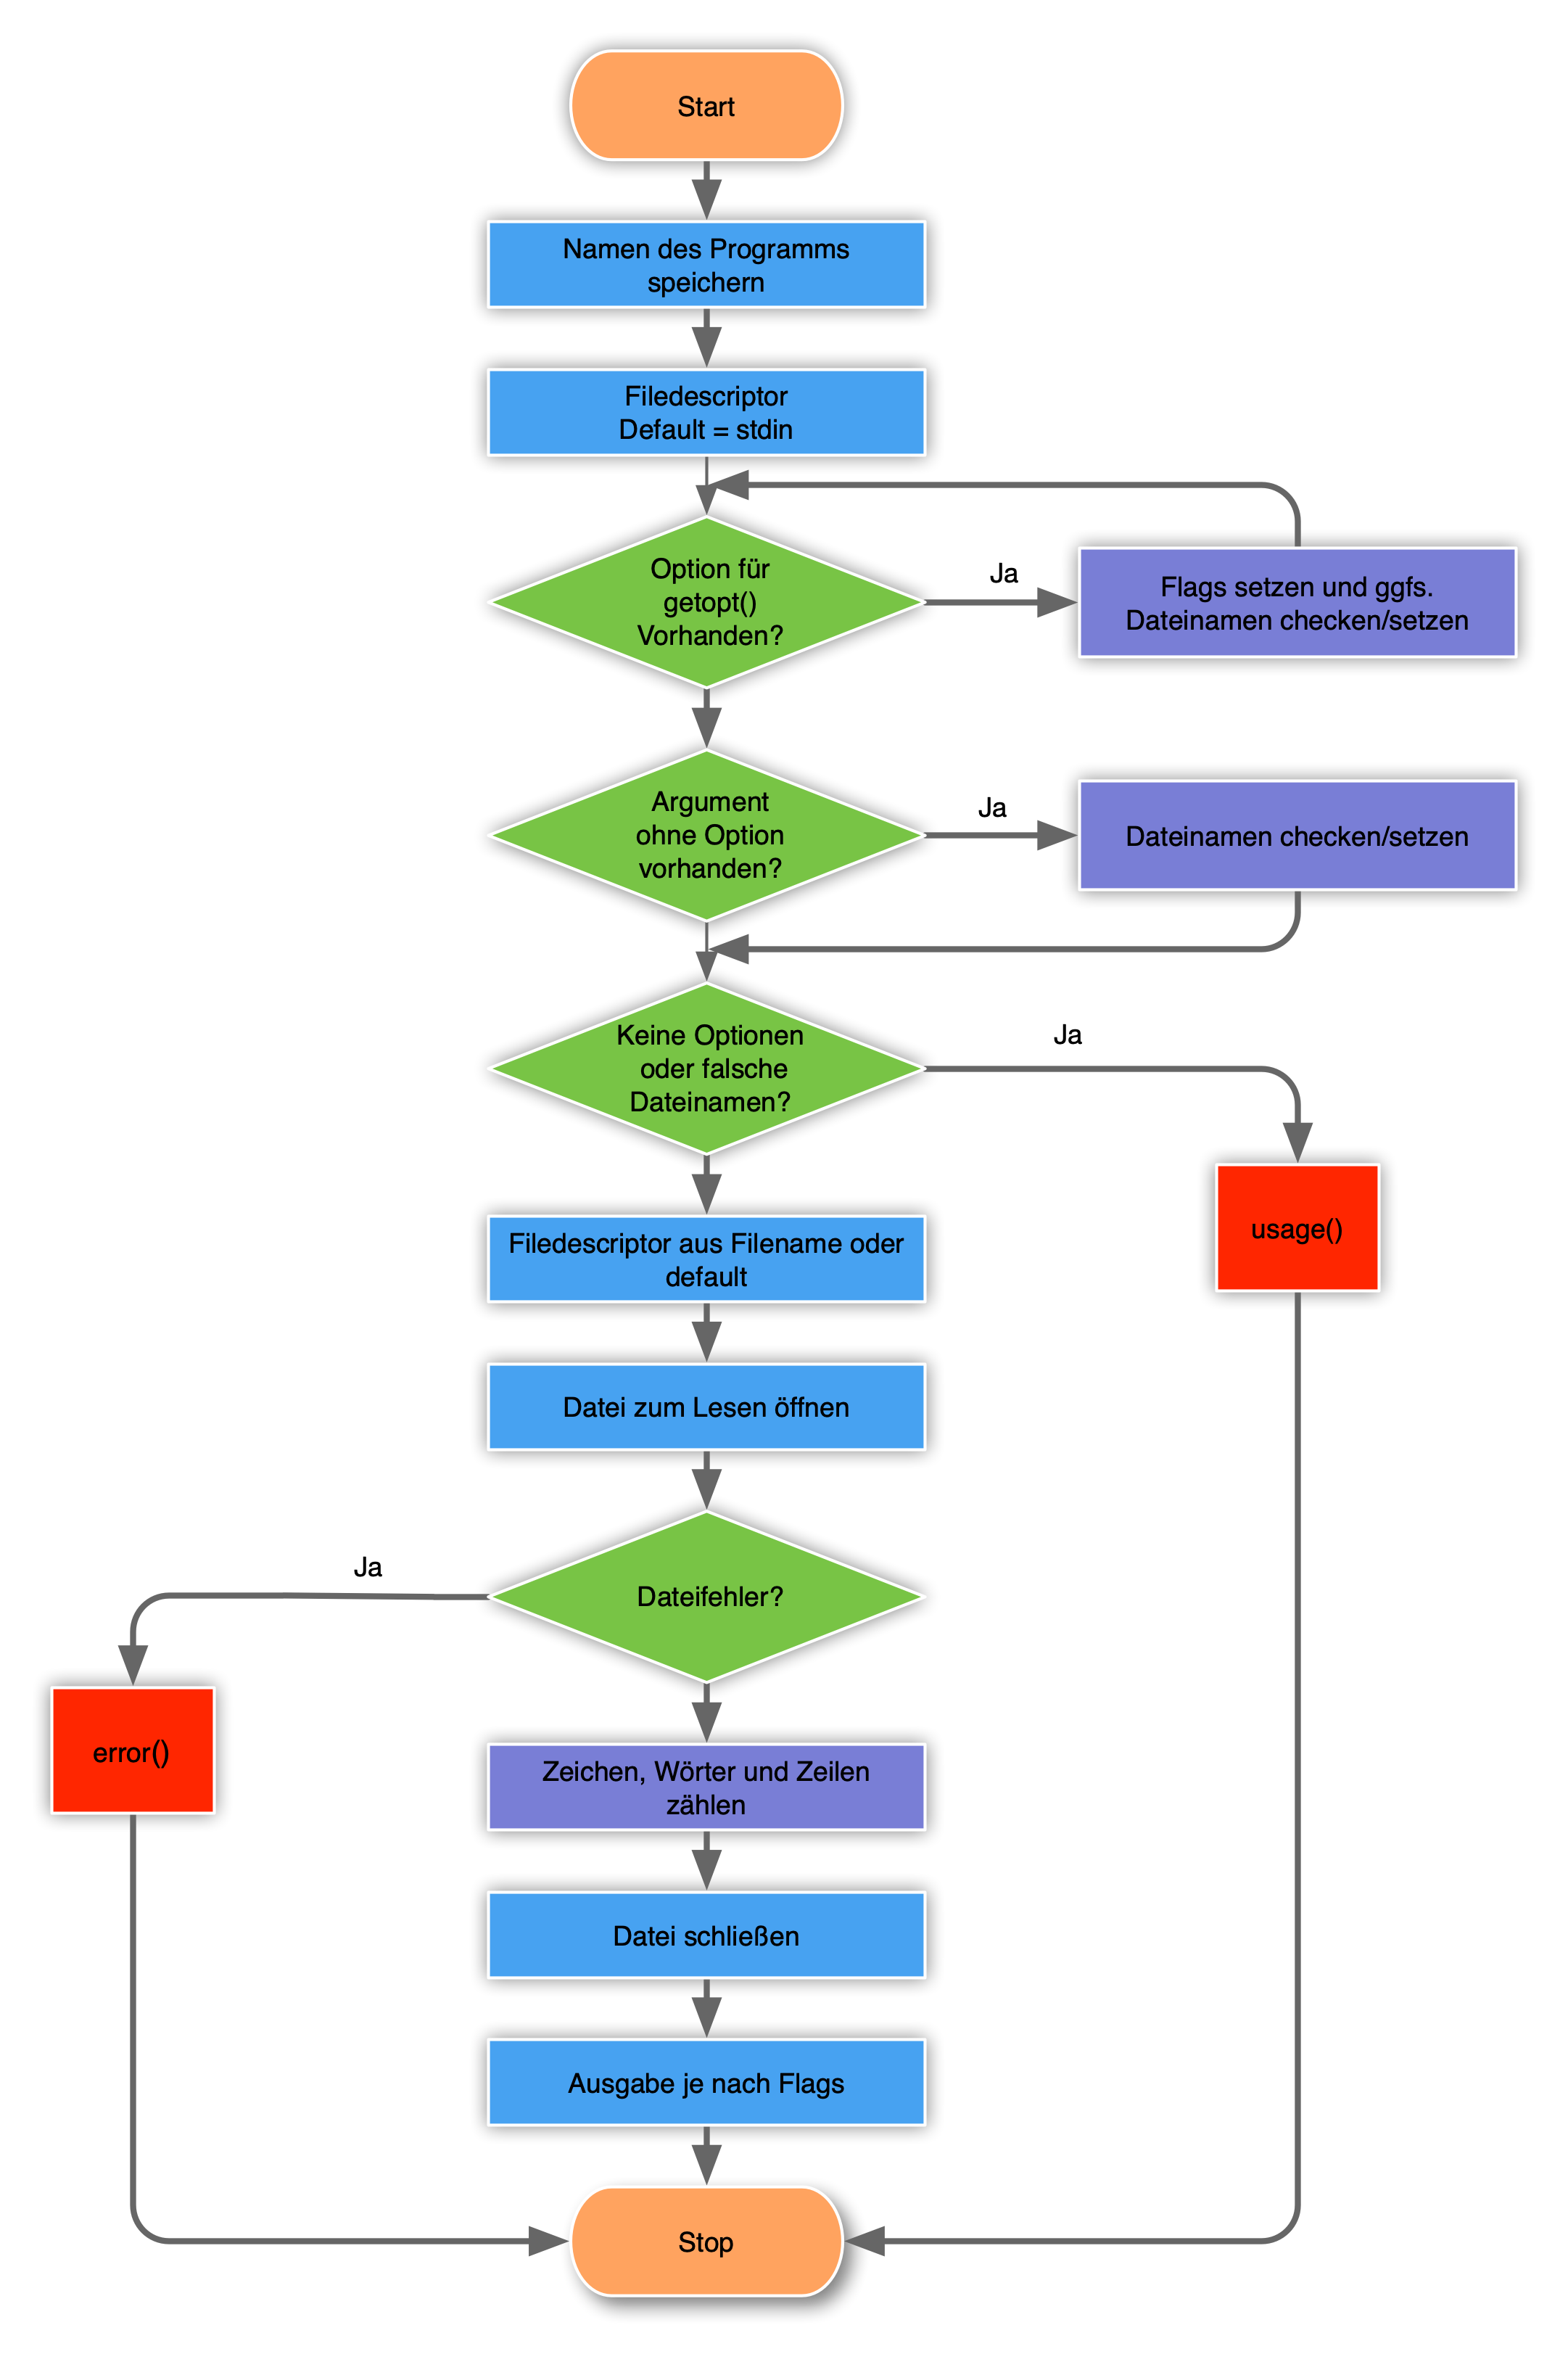
\includegraphics[height=9.2in]{Aufgabe01PAP.png}}
\lstset{ % General setup for the package
%     language={C},
%     basicstyle=\small\sffamily,
     numbers=left,
     numberstyle=\tiny,
%     frame=tb,
%     tabsize=4,
%     columns=fixed,
     showstringspaces=true,
     numbersep=5pt,
%     showtabs=false,
%     keepspaces,
     commentstyle=\color{olive},
     inputencoding=utf8/latin1
%     keywordstyle=\color{blue}
}%


\mylisting[label=musterloesung1]{Musterlösung1}{myfilter.c}
\mylisting[label=musterloesung2]{Musterlösung2}{Makefile}

\fi

\end{document}